% =====================================================================
\section{Matching a Vector Function to Its Curve}\label{ch:curves}
% =====================================================================

Multiple-choice items usually show four 3D curves and one formula, or one curve and four
formulas. You almost never need to plot. Run through the checklist below until only one
option is left; usually two or three steps are enough.

\begin{keybox}{The 7-step checklist for space curves $\vr(t)=\ip{x(t),y(t),z(t)}$}
\begin{enumerate}
\item \textbf{Are all components linear in $t$?} Then the curve is a \emph{straight line}
  (or a segment if $t$ is restricted).
\item \textbf{Find the ``circle pair''.} If two components are $a\cos t$ and $a\sin t$, then
  $x^2+y^2=a^2$: the curve lies on a \emph{cylinder} around the third axis, and viewed down
  that axis it is a circle. With $a\cos t,\ b\sin t$ it is an ellipse (elliptical cylinder).
\item \textbf{What does the third component do?}
  \begin{itemize}
  \item $=t$ (or $ct$): climbs steadily, so a \emph{helix} around that axis.
  \item periodic with the same period ($\sin t$, $\cos t$, $2-\sin t$): a \emph{closed loop}
    lying in a tilted plane, i.e.\ an \emph{ellipse}.
  \item $\cos 2t$, $\sin^2t$, \dots\ (twice as fast): \emph{2 ups and 2 downs} per turn (a
    ``pringle'' or saddle-shaped loop). $\cos nt$: $n$ ups per turn.
  \item $e^{ct}$: climbs faster and faster, so the coils get \emph{farther apart}.
  \item $\frac1{1+t^2}$: one bump near $t=0$, then flattens out (the curve circles at a
    nearly constant height).
  \end{itemize}
\item \textbf{Is the radius growing?} If the circle pair is $t\cos t,\ t\sin t$ then
  $x^2+y^2=t^2$; together with $z=t$ that is $x^2+y^2=z^2$: a \emph{cone} (conical helix).
  The variable that appears alone ($z=t$ here) is the axis of the cone.
\item \textbf{Look for algebraic relations.} $y=x^2$, $z=x^3$ (twisted cubic $\ip{t,t^2,t^3}$);
  $x+y=1$ (the curve lies in a plane); $x^2+y^2+z^2=$ const (the curve lies on a sphere).
\item \textbf{Check signs and bounds.} $t^2\ge0$ and $e^t>0$, so that coordinate is never
  negative. $\abs{\sin},\abs{\cos}\le1$ keep the curve inside a box. $\cos^2t,\sin^2t\in[0,1]$.
\item \textbf{Plug in $t=0$ (and maybe $t=\frac\pi2$).} This gives the starting point and
  usually eliminates the remaining look-alikes. For orientation, compare two values of $t$.
\end{enumerate}
\end{keybox}

\subsection*{Orientation and start point at a glance}

\begin{center}
\renewcommand{\arraystretch}{1.35}
\begin{tabular}{lll}
\toprule
\textbf{Pair $(x,y)$} & \textbf{Start ($t=0$)} & \textbf{Direction (viewed from above, $+z$)}\\
\midrule
$(\cos t,\ \sin t)$ & $(1,0)$ & counterclockwise\\
$(\sin t,\ \cos t)$ & $(0,1)$ & clockwise\\
$(\cos t,\ -\sin t)$ & $(1,0)$ & clockwise\\
$(-\cos t,\ \sin t)$ & $(-1,0)$ & clockwise\\
$(\cos(-t),\ \sin(-t))$ & $(1,0)$ & clockwise (reversing $t$ reverses direction)\\
\bottomrule
\end{tabular}
\end{center}

Rule: \emph{swapping} $\sin$ and $\cos$, or putting a minus sign on exactly one of them,
\emph{reverses} the direction.

\subsection*{Which axis is the curve wrapped around?}

The axis is the coordinate that is \emph{not} in the $\cos/\sin$ pair:
\[
\ip{\cos t,\sin t,t}\ \to\ z\text{-axis},\qquad
\ip{t,\cos t,\sin t}\ \to\ x\text{-axis},\qquad
\ip{\cos t,t,\sin t}\ \to\ y\text{-axis}.
\]

\subsection*{Projections onto the coordinate planes}
To see the curve ``from above'' drop $z$; ``from the front'' drop $y$; ``from the side'' drop $x$.
For the helix $\ip{\cos t,\sin t,t}$: from above a circle, from the side a sine wave
($y=\sin z$), from the front a cosine wave ($x=\cos z$). MC items sometimes show one of these
2D views instead of the 3D curve.

\subsection*{Gallery: formula $\to$ picture}

In each panel the red dot is the point at $t=0$ (or the left end of the interval) and the
thick red piece shows the direction of increasing $t$.

\begin{figure}[H]
  \centering
  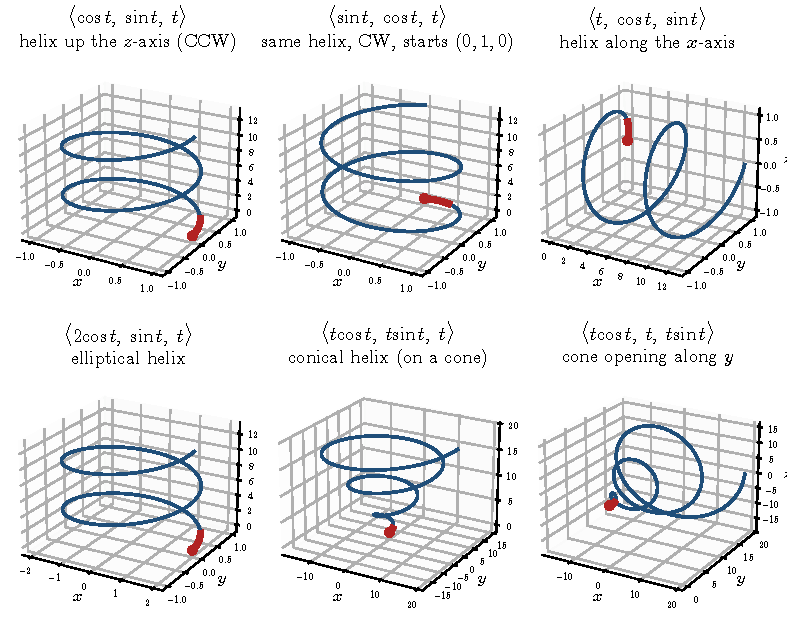
\includegraphics[width=\linewidth]{curves_gallery_1}
  \caption{Helices: circle pair + steadily increasing third component.
  The variable that appears alone is the axis.}
  \label{fig:curves1}
\end{figure}

\begin{figure}[H]
  \centering
  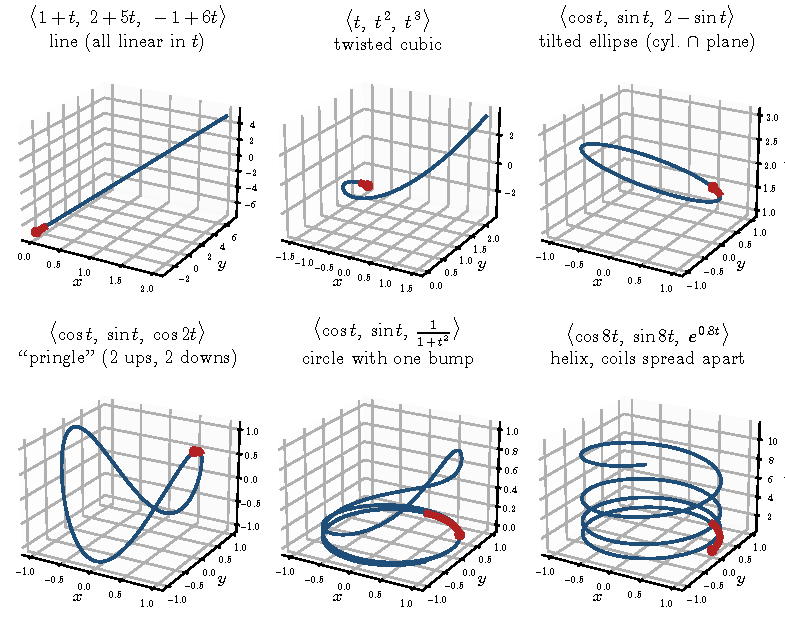
\includegraphics[width=\linewidth]{curves_gallery_2}
  \caption{Lines, the twisted cubic, closed loops on the cylinder $x^2+y^2=1$, and
  helices whose height is not linear in $t$.}
  \label{fig:curves2}
\end{figure}

\begin{figure}[H]
  \centering
  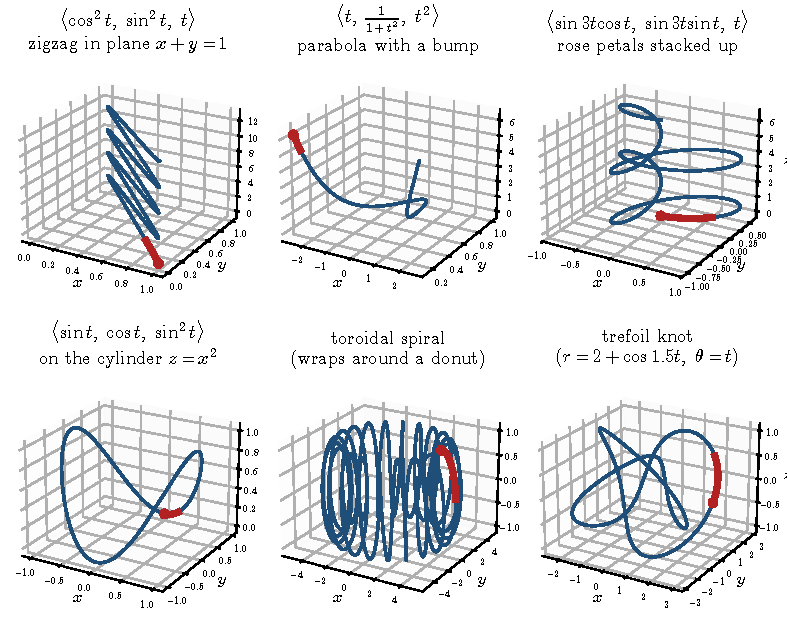
\includegraphics[width=\linewidth]{curves_gallery_3}
  \caption{More shapes that appear in matching items, including the two computer-drawn
  curves from the slides (toroidal spiral and trefoil knot).}
  \label{fig:curves3}
\end{figure}

\subsection*{Reverse look-up: picture $\to$ formula}

\begin{center}
\renewcommand{\arraystretch}{1.4}
\begin{tabularx}{\linewidth}{L{0.42\linewidth}Y}
\toprule
\textbf{If the picture shows\dots} & \textbf{look for a formula with\dots}\\
\midrule
a straight line & every component linear: $\ip{x_0+at,\ y_0+bt,\ z_0+ct}$\\
a spring with equal spacing & a $\cos t/\sin t$ pair and the third component $=ct$\\
a spring whose coils spread apart & third component growing faster than linear ($e^{t}$, $t^2$)\\
a spring that widens (cone) & pair $t\cos t,\ t\sin t$ (radius $=t$)\\
a flat closed loop, tilted & pair $\cos t,\sin t$ and third component $=a+b\cos t+c\sin t$\\
a closed loop going up--down--up--down & third component $\cos2t$, $\sin2t$, $\sin^2t$, $\cos^2t$\\
a circle with one bump that settles & third component $\frac1{1+t^2}$ (or $e^{-t^2}$)\\
an S-shaped curve through the origin & polynomial components like $\ip{t,t^2,t^3}$\\
a curve that stays on one side ($z\ge0$) & a component such as $t^2$, $e^t$, $\sin^2t$\\
a curve that wraps a donut & $\bigl((R+\sin nt)\cos t,\ (R+\sin nt)\sin t,\ \cos nt\bigr)$\\
\bottomrule
\end{tabularx}
\end{center}

\subsection*{2D curves from Topic 5 (parametric plane curves)}

\begin{center}
\renewcommand{\arraystretch}{1.35}
\begin{tabularx}{\linewidth}{L{0.42\linewidth}Y}
\toprule
\textbf{Parametrization} & \textbf{Curve}\\
\midrule
$\ip{h+r\cos t,\ k+r\sin t}$ & circle, centre $(h,k)$, radius $r$, CCW\\
$\ip{a\cos t,\ b\sin t}$ & ellipse $\frac{x^2}{a^2}+\frac{y^2}{b^2}=1$\\
$\ip{t,\ f(t)}$ & the graph $y=f(x)$\\
$\ip{t^2-2t,\ t+1}$ (slides) & eliminate $t$: $t=y-1$, $x=(y-1)^2-2(y-1)$, a sideways parabola\\
$\ip{a\cosh t,\ b\sinh t}$ & right branch of a hyperbola ($\cosh^2-\sinh^2=1$)\\
\bottomrule
\end{tabularx}
\end{center}
To identify a plane curve, \emph{eliminate $t$}: use $\cos^2t+\sin^2t=1$ for trig pairs, or
solve one equation for $t$ and substitute into the other.
